\Variant{25.05.2025 (2-smena)}
\QQ{1}{Agar $a,b\in\mathbb N$, $a\cdot b=2^3\cdot3^5\cdot7^2$ bölsa, EKUK$(a;\,b)$ ning eng kiçik qiymatini toping.
\Opts{$756$}{$588$}{$786$}{$420$}}
\QQ{2}{Agar $a=\sqrt[3]{12}$, $b=\sqrt6$, $c=2\sqrt[6]3$ bölsa, $\dfrac{|a-b|+|b-c|-|a-c|-|2a|}{|a+c-b|}$ ni soddalaştiring.
\Opts{$1$}{$-1$}{$2$}{$-2$}}
\QQ{3}{Ikki sohil orasidagi masofa $24$ km ga teng. Motorli qayiq borib kelişi uçun $9$ soat vaqt sarfladi. Oqim tezligi $2$ km/soat ga teng bölsa, motorli qayiqning turğun suvdagi tezligi oqim tezligidan neça marta katta?
\Opts{$2$}{$3$}{$4$}{$6$}}
\QQ{4}{$6$ ta bir xil şişa idişning hajmi $2$ ta boçka hajmining $90\%$ iga teng bölsa, $1$ ta şişa idiş hajmi $1$ ta boçka hajmining neça foiziga teng.
\Opts{$15\%$}{$20\%$}{$40\%$}{$30\%$}}
\QQ{5}{Hisoblang:
\[(0{,}25)^{-\frac12}\cdot3^{-1}+(0{,}5)^{-2}\cdot9^{-\frac12}\]
\Opts{$2$}{$\dfrac12$}{$3$}{$\dfrac13$}}
\QQ{6}{Hisoblang:
\[\frac4{\sqrt{13}+3}-\frac9{\sqrt{13}-2}\]
\Opts{$5$}{$2\sqrt{13}$}{$-2\sqrt{13}$}{$-5$}}
\QQ{7}{Hisoblang:
\[\sqrt[3]{2+\sqrt5}+\sqrt[3]{2-\sqrt5}\]
\Opts{$-1$}{$\sqrt2$}{$1$}{$2$}}
\QQ{8}{Arifmetik progressiyada $a_4+a_{17}=17$, $S_{14}-S_3=77$, $a_k=2023$ bölsa, $\sqrt k$ ning qiymatini toping.
\Opts{$2025$}{$45$}{$\sqrt{2024}$}{$\sqrt{2023}$}}
\QQ{9}{Geometrik progressiyada $b_4-b_1=52$, $b_7-b_1=1456$ bölsa, $S_6$ ning qiymatini toping.
\Opts{$532$}{$272$}{$736$}{$728$}}
\QQ{10}{Agar $x=6$ bölsa, $\left(\dfrac1{\sqrt x+\sqrt2}-\dfrac1{\sqrt x-\sqrt2}\right)^{-2}$ ni hisoblang.
\Opts{$2$}{$3$}{$\dfrac12$}{$4$}}
\QQ{11}{$\dfrac1{\sqrt3+\sqrt4}+\dfrac1{\sqrt4+\sqrt5}+\dots+\dfrac1{\sqrt{24}+\sqrt{25}}$ soni qaysi oraliqqa tegişli?
\Opts{$(4;\,5)$}{$(2;\,3)$}{$(3;\,4)$}{$(1;\,3)$}}
\QQ{12}{Hisoblang:
\[\tg\left(\arcsin\left(-\frac12\right)\right)\]
\Opts{$-\sqrt3$}{$-\dfrac{\sqrt3}3$}{$\sqrt3$}{$\dfrac{\sqrt3}3$}}
\QQ{13}{$\dfrac{3\left(x-5\sqrt x+6\right)}{x-4}>\sqrt x-3$ tengsizlikning butun yeçimlari yiğindisini toping.
\Opts{$29$}{$31$}{$30$}{$28$}}
\QQ{14}{$25\cdot2^x-10^x+5^x\ge25$ tengsizlikning butun yeçimlari yiğindisini toping.
\Opts{$0$}{$2$}{$3$}{$4$}}
\QQ{15}{Tenglamalar sistemasi neçta haqiqiy $(x;\,y)$ juftligiga ega?
\[\begin{cases}\sqrt{x+y}+\sqrt{x-y}=y,\\ x^2=y^2+36\end{cases}\]
\Opts{$1$}{$2$}{$3$}{$4$}}
\QQ{16}{$2\lg2+\left(1+\dfrac1{2x}\right)\lg3=\lg\left(3^{\frac1x}+27\right)$ tenglamaning barça haqiqiy ildizlari yiğindisini toping (agar u bitta bölsa, şu ildizni toping).
\Opts{$\dfrac12$}{$\dfrac34$}{$\dfrac43$}{$\dfrac23$}}
\QQ{17}{$\sqrt{\ctg x}\cdot(2\sin x-1)=0$ tenglamaning $[0;\,2\pi]$ oraliğidagi ildizlari yiğindisini toping.
\Opts{$2\pi$}{$\dfrac{10\pi}3$}{$\dfrac{13\pi}6$}{$\pi$}}
\QQ{18}{Tengsizlikning butun yeçimlari yiğindisini toping:
\[\sqrt{x-2}-\sqrt[4]{6-x}\ge0\]
\Opts{$10$}{$9$}{$15$}{$12$}}
\QQ{19}{$\sqrt{3x-x^2+4}=a$ tenglama $a$ ning neçta butun qiymatida yeçimga ega böladi?
\Opts{$7$}{$3$}{$4$}{$2$}}
\QQ{20}{$f(x)=x+3$ bölsa, $3\big(f(2x)-2f(x-1)\big)$ ning qiymatini toping.
\Opts{$-3$}{$3$}{$1$}{$4$}}
\QQ{21}{$af(x)+bf\left(\dfrac1x\right)=\dfrac1x-2024$ bölsa, $f(x)$ ni toping. $a\ne0$, $b\ne0$, $a\ne\pm b$.
\Opts{$f(x)=\dfrac1{a^2-b^2}\left(\dfrac ax+bx\right)-\dfrac{2024}{a+b}$}{$f(x)=\dfrac1{a^2-b^2}\left(\dfrac ax-bx\right)-\dfrac{2024}{a+b}$}{$f(x)=\dfrac1{a^2-b^2}\left(\dfrac ax-bx\right)+\dfrac{2024}{a+b}$}{$f(x)=\dfrac1{a^2-b^2}\left(\dfrac ax+bx\right)+\dfrac{2024}{a+b}$}}
\QQ{22}{$y=\dfrac1{1-\cos x}+\dfrac4{\cos x}$ funksiyaning $\left[\dfrac\pi6;\,\dfrac\pi3\right]$ oraliqdagi eng kiçik qiymatini toping.
\Opts{$10$}{$8$}{$7$}{$9$}}
\QQ{23}{Hisoblang:
\[\int_0^{\frac\pi4}\frac{\sin^6x}{\cos^8x}\,dx\]
\Opts{$\dfrac17$}{$\dfrac56$}{$\dfrac27$}{$\dfrac37$}}
\QQ{24}{Kvadratga aylana içki çizilgan. Kvadrat perimetrining aylana uzunligiga nisbatini toping.
\Opts{$\dfrac4\pi$}{$\dfrac2\pi$}{$\dfrac1\pi$}{$\dfrac6\pi$}}
\QQ{25}{$ABCDEF$ — muntazam oltiburçak, $CE$ va $AF$ töğri çiziqlar $G$ nuqtada kesişadi, $FG=6$ cm. Ştrixlangan soha yuzini toping.
\qfig{\begin{tikzpicture}[scale=0.38,font=\small]
\coordinate (A) at (0,0); \coordinate (F) at (3,0); \coordinate (E) at (4.5,2.598); \coordinate (D) at (3,5.196); \coordinate (C) at (0,5.196); \coordinate (B) at (-1.5,2.598); \coordinate (G) at (9,0);
\fill[qfill] (A)--(C)--(E)--(F)--cycle;
\draw (A)--(B)--(C)--(D)--(E)--(F)--cycle; \draw (A)--(C)--(G)--(F);
\node[below left] at (A) {$A$}; \node[left] at (B) {$B$}; \node[above left] at (C) {$C$}; \node[above right] at (D) {$D$}; \node[above right] at (E) {$E$}; \node[below] at (F) {$F$}; \node[below right] at (G) {$G$};
\node[below] at (6,0) {$6$ cm};
\end{tikzpicture}}
\Opts{$12\sqrt3$}{$9\sqrt3$}{$6\sqrt3$}{$18\sqrt3$}}
\QQ{26}{$ABC$ töğri burçakli uçburçakka taşqi çizilgan aylana radiusi $R=25$, içki çizilgan aylana radiusi $r=5$ bölsa, $ABC$ uçburçak yuzini toping.
\qfig{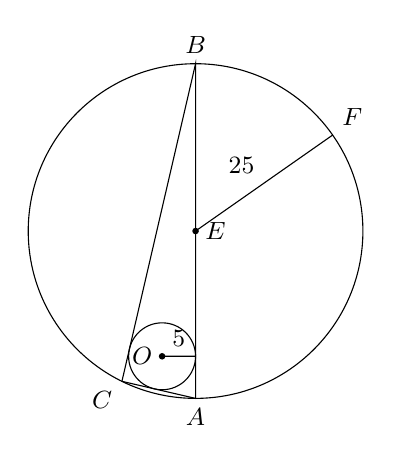
\begin{tikzpicture}[scale=0.085,font=\small]
\coordinate (E) at (0,0); \coordinate (A) at (0,-25); \coordinate (B) at (0,25); \coordinate (C) at (-11,-22.45); \coordinate (O) at (-5,-18.71); \coordinate (F) at (20.48,14.34);
\draw (E) circle (25); \draw (A)--(B)--(C)--cycle; \draw (O) circle (5); \draw (E)--(F); \draw (O)--(0,-18.71);
\fill (E) circle (14pt); \fill (O) circle (14pt);
\node[above] at (B) {$B$}; \node[below] at (A) {$A$}; \node[below left] at (C) {$C$}; \node[right] at (E) {$E$}; \node[above right] at (F) {$F$}; \node[left] at (O) {$O$};
\node[above left] at (10.24,7.17) {$25$}; \node[above] at (-2.5,-18.71) {$5$};
\end{tikzpicture}}
\Opts{$225$}{$250$}{$245$}{$275$}}
\QQ{27}{$ABCD$ kvadrat. $MNC$ — töğri burçakli uçburçak. Agar $CN=4$, $MN=3$ va $CM=5$ bölsa, $ABCD$ kvadrat yuzini toping.
\qfig{\begin{tikzpicture}[scale=0.85,font=\small]
\coordinate (A) at (0,0); \coordinate (B) at (0,3.88); \coordinate (C) at (3.88,3.88); \coordinate (D) at (3.88,0); \coordinate (N) at (2.91,0); \coordinate (M) at (0,0.728);
\draw (A)--(B)--(C)--(D)--cycle; \draw (M)--(N)--(C)--cycle;
\draw ($(N)!0.22cm!(M)$)--($(N)!0.22cm!(M)+(N)!0.22cm!(C)-(N)$)--($(N)!0.22cm!(C)$);
\node[below left] at (A) {$A$}; \node[above left] at (B) {$B$}; \node[above right] at (C) {$C$}; \node[below right] at (D) {$D$}; \node[below] at (N) {$N$}; \node[left] at (M) {$M$};
\node[above] at (1.4,0.4) {$3$}; \node[right] at (3.4,1.9) {$4$}; \node[above left] at (1.94,2.3) {$5$};
\end{tikzpicture}}
\Opts{$15\dfrac1{17}$}{$16\dfrac1{17}$}{$17$}{$20$}}
\QQ{28}{$ABC$ — töğri burçakli uçburçak ($\angle C=90^\circ$). $AD=4$, $CD=6$, $DE=EB=5$ bölsa, ştrixlangan yuzni toping.
\qfig{\begin{tikzpicture}[scale=0.34,font=\small]
\coordinate (C) at (0,0); \coordinate (A) at (10,0); \coordinate (D) at (6,0); \coordinate (B) at (0,8); \coordinate (E) at (3,4);
\fill[qfill] (B)--(E)--(A)--cycle;
\draw (A)--(B)--(C)--cycle; \draw (B)--(D); \draw (E)--(A); \draw (0,0.6)--(0.6,0.6)--(0.6,0);
\node[below left] at (C) {$C$}; \node[below right] at (A) {$A$}; \node[below] at (D) {$D$}; \node[above left] at (B) {$B$}; \node[left] at (E) {$E$};
\node[below] at (3,0) {$6$}; \node[below] at (8,0) {$4$}; \node[left] at (1.5,6) {$5$}; \node[left] at (4.5,2) {$5$};
\end{tikzpicture}}
\Opts{$16$}{$2$}{$6$}{$8$}}
\QQ{29}{$ABCD$ — teng yonli trapetsiya. $\dfrac{BC}{AD}=\dfrac13$, $MN$ — örta çiziq, $BH$ balandligi $MN$ ni $O$ nuqtada kesadi. $\overrightarrow{AO}=a\cdot\overrightarrow{AB}+b\cdot\overrightarrow{BC}$ bölsa, $\dfrac ab$ ning qiymatini toping.
\qfig{\begin{tikzpicture}[scale=0.8,font=\small]
\coordinate (A) at (0,0); \coordinate (D) at (6,0); \coordinate (B) at (2,2.4); \coordinate (C) at (4,2.4); \coordinate (H) at (2,0); \coordinate (M) at (1,1.2); \coordinate (N) at (5,1.2); \coordinate (O) at (2,1.2);
\draw (A)--(B)--(C)--(D)--cycle; \draw (M)--(N); \draw (B)--(H); \draw[-{Stealth[length=5pt]}] (A)--(O); \draw (2,0.3)--(2.3,0.3)--(2.3,0);
\node[below left] at (A) {$A$}; \node[below right] at (D) {$D$}; \node[above left] at (B) {$B$}; \node[above right] at (C) {$C$}; \node[below] at (H) {$H$}; \node[left] at (M) {$M$}; \node[right] at (N) {$N$}; \node[above right] at (O) {$O$};
\end{tikzpicture}}
\Opts{$\dfrac12$}{$\dfrac34$}{$1$}{$\dfrac43$}}
\QQ{30}{Konus töla sirti asosining yuzidan $8$ marta katta. Konus balandligi $24$ ga teng bölsa, konus hajmini toping.
\Opts{$108\pi$}{$96\pi$}{$72\pi$}{$64\pi$}}
\QQ{31}{Bu yerda $a$, $b$, $c$ — turli raqamlar. $\underbrace{\overline{abcabc\ldots abc}}_{2025\ \text{xonali}}$ körinişdagi $2025$ xonali sonlar neçta?
\Opts{$1000$}{$900$}{$720$}{$648$}}
\QQ{32}{$A=\{x\mid2\le x\le4,\ x\in\mathbb R\}$, $B=\{x\mid6\le x\le8,\ x\in\mathbb R\}$, $C=\{x\mid3\le x\le7,\ x\in\mathbb R\}$, $D=\{x\mid3\le x\le4,\ x\in\mathbb R\}$, $E=\{x\mid6\le x\le7,\ x\in\mathbb R\}$ töplamlar berilgan. Quyidagi töplamlardan qaysi biri $D\cup E$ töplamga teng böladi?
\Opts{$(A\cap B)\cap C$}{$(A\cup B)\cap C$}{$(A\cap B)\cup C$}{$(A\cup B)\cup C$}}
\QQ{33}{\Moslash{Rasmda uçlari $A(-3;\,2)$, $B\left(-1;\,2\sqrt3+2\right)$, $C\left(3;\,2\sqrt3+2\right)$, $D(9;\,2)$ nuqtalarda bölgan törtburçak berilgan.
\par\centering\begin{tikzpicture}[x=0.36cm,y=0.36cm,font=\small]
\draw[-{Stealth[length=4pt]}] (-5,0)--(11,0) node[right] {$x$}; \draw[-{Stealth[length=4pt]}] (0,-0.8)--(0,7) node[right] {$y$};
\draw (-3,2)--(-1,5.46)--(3,5.46)--(9,2)--cycle;
\node[left] at (-3,2) {$A$}; \node[above] at (-1,5.46) {$B$}; \node[above] at (3,5.46) {$C$}; \node[right] at (9,2) {$D$}; \node[below left] at (0,0) {$O$};
\end{tikzpicture}}{A) $81\sqrt3$\par B) $16\sqrt3$\par C) $80\pi$\par D) $48\sqrt3$\par E) $72\left(\sqrt3+1\right)$\par F) $24\left(\sqrt3+1\right)\pi$}{$ABCD$ trapetsiya yuzini hisoblang.}{$ABCD$ törtburçakning katta tomoni atrofida $360^\circ$ ga aylantirişdan hosil bölgan jismning töla sirtini toping.}{$ABCD$ törtburçakning katta tomoni atrofida $360^\circ$ ga aylantirişdan hosil bölgan jismning hajmini toping.}}
\QQ{36}{Tenglamani yeçing:
\[\left(99+70\sqrt2\right)^x-7\left(17+12\sqrt2\right)^x+8\left(3+2\sqrt2\right)^x+\left(3-2\sqrt2\right)^x=7\]
\AB{Tenglama neçta haqiqiy ildizga ega?}{Tenglamaning haqiqiy ildizlari yiğindisini toping.}}
\QQ{37}{Tenglamani yeçing:
\[\left(2\sin x-\sqrt3\right)\cdot\sqrt{7x-4-3x^2}=0\]
\AB{Tenglama neçta haqiqiy ildizga ega?}{Tenglamaning eng katta va eng kiçik ildizlari köpaytmasini toping.}}
\QQ{38}{$f(x)=a\cdot x^n+b$ funksiya uçun $n\in\mathbb N$, $f(x)\cdot f\left(\dfrac1x\right)=f(x)+f\left(\dfrac1x\right)$ va $f(3)=82$ tenglik örinli bölsa,
\AB{$f(2)+f(1)$ ning qiymatini toping.}{$y=f(x)$ funksiyaning qiymatlar sohasini toping.}}
\QQ{39}{$f(x)=\sin\left(\dfrac1x\right)$ funksiya berilgan.
\AB{$f'\left(\dfrac1\pi\right)$ ning qiymatini toping.}{$g(x)=f(x)+2x^3f'(x)+x^4f''(x)$ bölsa, $g(2025)$ ning qiymatini toping.}}
\QQ{40}{$f(x)$ funksiya uçun $\displaystyle\int_0^1f(x)\cdot f'(x)\,dx=0$ va $\displaystyle\int_0^1f^2(x)\cdot f'(x)\,dx=18$ tenglik örinli bölsa,
\AB{$f(1)$ ni toping.}{$\displaystyle\int_0^1f^4(x)\cdot f'(x)\,dx$ ning qiymatini toping.}}
\QQ{41}{Rasmda $ABCD$ töğri törtburçak tasvirlangan bölib, bunda $S_{ABK}=15$, $S_{FEG}=4$, $S_{AFD}=15$, $S_{KHG}=S_1$ va $S_{AKGF}=S_2$ ga teng bölsa,
\qfig{\begin{tikzpicture}[scale=0.42,font=\small]
\coordinate (A) at (0,0); \coordinate (B) at (0,10); \coordinate (C) at (11,10); \coordinate (D) at (11,0); \coordinate (H) at (3.667,10); \coordinate (E) at (11,3.333);
\coordinate (K) at (3,8.182); \coordinate (G) at (6.6,6); \coordinate (F) at (9,2.727);
\fill[qfill!55] (K)--(H)--(G)--cycle; \fill[qfill] (A)--(K)--(G)--(F)--cycle; \fill[qfill!80!black!30] (F)--(E)--(G)--cycle;
\draw (A)--(B)--(C)--(D)--cycle; \draw (A)--(H)--(D); \draw (B)--(E)--(A);
\node[below left] at (A) {$A$}; \node[above left] at (B) {$B$}; \node[above right] at (C) {$C$}; \node[below right] at (D) {$D$}; \node[above] at (H) {$H$}; \node[right] at (E) {$E$};
\node[left] at (K) {$K$}; \node[above right] at (G) {$G$}; \node[below] at (F) {$F$};
\node at (4.45,8.1) {\scriptsize$S_1$}; \node at (5,5) {$S_2$}; \node at (1.3,6.3) {$15$}; \node at (7.5,1.6) {$15$}; \node at (9.1,4.15) {\scriptsize$4$};
\end{tikzpicture}}
\AB{$S_1$ ni toping.}{$AB=10$ va $AD=11$ ga teng bölsa, $S_2$ ni toping.}}
\QQ{42}{$ABC$ uçburçakning $a$, $b$, $c$ tomonlariga tuşirilgan balandliklari mos ravişda $h_a=12$, $h_b=12\dfrac{12}{13}$ va $h_c=11\dfrac15$ ga teng.
\AB{$ABC$ uçburçakka içki çizilgan aylana radiusini toping.}{$ABC$ uçburçakning yuzini toping.}}
\QQ{43}{$ABCDEF$ muntazam oltiburçakning yuzi $6\sqrt3$ ga teng. $CE$, $AD$, $BE$ va $DF$ kesmalar ötkazilgan: $K=CE\cap AD$, $L=AD\cap BE$, $M=BE\cap DF$, $N=CE\cap DF$.
\qfig{\begin{tikzpicture}[scale=0.95,font=\small]
\coordinate (L) at (0,0); \coordinate (B) at (-2,0); \coordinate (E) at (2,0); \coordinate (C) at (-1,1.732); \coordinate (D) at (1,1.732); \coordinate (A) at (-1,-1.732); \coordinate (F) at (1,-1.732);
\coordinate (K) at (0.5,0.866); \coordinate (N) at (1,0.577); \coordinate (M) at (1,0);
\fill[qfill] (L)--(K)--(N)--(M)--cycle;
\draw (A)--(B)--(C)--(D)--(E)--(F)--cycle; \draw (C)--(E); \draw (A)--(D); \draw (B)--(E); \draw (D)--(F);
\node[below left] at (A) {$A$}; \node[left] at (B) {$B$}; \node[above left] at (C) {$C$}; \node[above] at (D) {$D$}; \node[right] at (E) {$E$}; \node[below] at (F) {$F$};
\node[above left] at (K) {$K$}; \node[above left] at (L) {$L$}; \node[below right] at (M) {$M$}; \node[right] at (N) {$N$};
\end{tikzpicture}}
\AB{$LM$ kesma uzunligini toping.}{Ştrixlangan $LKNM$ soha yuzini toping.}}
\QQ{44}{Rasmda şar, konus va silindr tasvirlangan. Bunda $R_{\text{şar}}=R_{\text{konus}}=R_{\text{silindr}}$, $H_{\text{konus}}=H_{\text{silindr}}=H$ va $V_{\text{silindr}}=V_{\text{konus}}+V_{\text{şar}}$.
\qfig{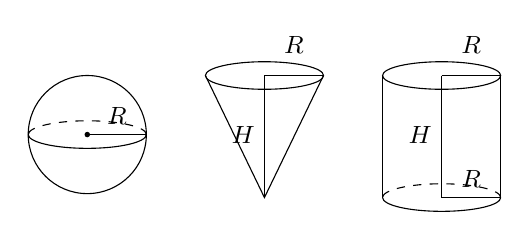
\begin{tikzpicture}[scale=0.5,font=\small]
\draw (0,0) circle (1.5); \draw (-1.5,0) arc (180:360:1.5 and 0.35); \draw[dashed] (1.5,0) arc (0:180:1.5 and 0.35); \fill (0,0) circle (2pt); \draw (0,0)--(1.5,0); \node[above] at (0.75,0) {$R$};
\begin{scope}[xshift=4.5cm]
\draw (0,1.5) ellipse (1.5 and 0.35); \draw (-1.5,1.5)--(0,-1.6)--(1.5,1.5); \draw (0,1.5)--(0,-1.6); \draw (0,1.5)--(1.5,1.5);
\node[above] at (0.75,1.8) {$R$}; \node[left] at (0,0) {$H$};
\end{scope}
\begin{scope}[xshift=9cm]
\draw (0,1.5) ellipse (1.5 and 0.35); \draw (-1.5,1.5)--(-1.5,-1.6); \draw (1.5,1.5)--(1.5,-1.6);
\draw (-1.5,-1.6) arc (180:360:1.5 and 0.35); \draw[dashed] (1.5,-1.6) arc (0:180:1.5 and 0.35);
\draw (0,1.5)--(0,-1.6)--(1.5,-1.6); \draw (0,1.5)--(1.5,1.5);
\node[above] at (0.75,1.8) {$R$}; \node[left] at (0,0) {$H$}; \node[above] at (0.75,-1.6) {$R$};
\end{scope}
\end{tikzpicture}}
\AB{Agar $H=10$ cm ga teng bölsa, silindrsimon idişga neça litr suv ketadi?}{Şar sirti yuzi $144\pi$ ga teng bölsa, silindrning hajmini toping.}}
\QQ{45}{Rasmdagi körsatilgan doira $1:2$ nisbatda kiçik va katta sektorlarga bölingan. Kiçik sektordan 1-stakan (konus), katta sektordan 2-stakan (konus) yasalgan bölsa,
\qfig{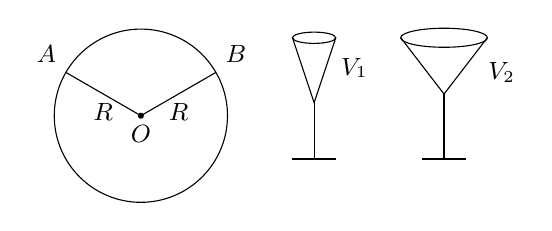
\begin{tikzpicture}[scale=0.55,font=\small]
\coordinate (O) at (0,0); \coordinate (A) at (-1.732,1); \coordinate (B) at (1.732,1);
\draw (O) circle (2); \draw (A)--(O)--(B); \fill (O) circle (2pt);
\node[below] at (O) {$O$}; \node[above left] at (A) {$A$}; \node[above right] at (B) {$B$}; \node[below] at (-0.87,0.5) {$R$}; \node[below] at (0.87,0.5) {$R$};
\begin{scope}[xshift=4cm,yshift=0.6cm]
\draw (0,1.2) ellipse (0.5 and 0.13); \draw (-0.5,1.2)--(0,-0.3)--(0.5,1.2); \draw (0,-0.3)--(0,-1.6); \draw (-0.5,-1.6)--(0.5,-1.6); \node[right] at (0.4,0.5) {$V_1$};
\end{scope}
\begin{scope}[xshift=7cm,yshift=0.6cm]
\draw (0,1.2) ellipse (1 and 0.22); \draw (-1,1.2)--(0,-0.1)--(1,1.2); \draw (0,-0.1)--(0,-1.6); \draw (-0.5,-1.6)--(0.5,-1.6); \node[right] at (0.8,0.4) {$V_2$};
\end{scope}
\end{tikzpicture}}
\AB{1-stakan hajmining 2-stakan hajmiga nisbatini toping.}{1-konusga içki çizilgan şar hajmining 2-konusga içki çizilgan şar hajmiga nisbatini toping.}}
\Javoblar{A D B D A D C B D A C B B C A B C C B A B D A A B D A D C B D B B F C}{%
\OK{36}{$2$}{$0$}\OK{37}{$3$}{$\dfrac43$}\OK{38}{$19$}{$[1;\,\infty)$}\OK{39}{$\pi^2$}{$0$}\OK{40}{$3$}{$\dfrac{486}5$}%
\OK{41}{$4$}{$36$}\OK{42}{$4$}{$84$}\OK{43}{$1$}{$\dfrac{\sqrt3}3$}\OK{44}{$\dfrac\pi4\approx0{,}785$}{$432\pi$}\OK{45}{$\dfrac{\sqrt{10}}{10}$}{$\dfrac{5\sqrt{10}}{32}$}}
